% =============================================================================
% CHƯƠNG 5: KẾT QUẢ ĐO LƯỜNG VÀ PHÂN TÍCH
% =============================================================================
\chapter{Kết quả đo lường và phân tích}

\section{Phương pháp đo lường}

Các thí nghiệm được thực hiện trên cùng một topology MPLS backbone, chỉ thay đổi kiến trúc LAN tại chi nhánh để đảm bảo tính so sánh công bằng:

\begin{itemize}
    \item \textbf{Throughput}: Đo bằng \texttt{iperf3} chế độ TCP, thời gian 10 giây, giữa các cặp host thuộc chi nhánh khác nhau.
    \item \textbf{Delay (RTT)}: Đo bằng lệnh \texttt{ping}, 50 gói ICMP, ghi lại min/avg/max và mdev.
    \item \textbf{Packet Loss}: Ghi nhận từ output ping (\%) và iperf3 UDP.
    \item \textbf{Jitter}: Tính từ \texttt{mdev} (mean deviation) trong ping, hoặc \texttt{jitter\_ms} từ iperf3 UDP.
\end{itemize}

Mỗi kịch bản được lặp lại \textbf{3 lần} và lấy giá trị trung bình.

\section{Kết quả đo lường}

\subsection{Bảng tổng hợp số liệu}

\begin{table}[htbp]
    \centering
    \caption{Bảng tổng hợp kết quả đo lường hiệu năng (giá trị trung bình)}
    \vspace{0.2cm}
    \small
    \begin{tabularx}{\textwidth}{|>{\raggedright\arraybackslash}p{1.2cm}|>{\raggedright\arraybackslash}p{2.5cm}|c|c|c|c|}
        \hline
        \textbf{Kịch bản} & \textbf{Kiến trúc LAN} & \textbf{Throughput (Mbps)} & \textbf{Delay (ms)} & \textbf{Loss (\%)} & \textbf{Jitter (ms)} \\ \hline
        SC-1 & Flat Network & \textbf{94.2} & 0.82 & 0.0 & 0.041 \\ \hline
        SC-2 & 3-Tier (Core–Dist–Acc) & 88.7 & 1.24 & 0.0 & 0.063 \\ \hline
        SC-3 & Leaf-Spine & \textbf{97.5} & \textbf{0.61} & 0.0 & \textbf{0.028} \\ \hline
    \end{tabularx}
\end{table}

\begin{table}[htbp]
    \centering
    \caption{Chi tiết kết quả từng cặp host đo lường trong 3 kịch bản}
    \vspace{0.2cm}
    \small
    \begin{tabularx}{\textwidth}{|c|c|c|c|c|c|}
        \hline
        \textbf{Kịch bản} & \textbf{Src → Dst} & \textbf{Throughput (Mbps)} & \textbf{RTT avg (ms)} & \textbf{RTT min (ms)} & \textbf{Packet Loss (\%)} \\ \hline
        \multirow{2}{*}{SC-1} & h1a → h2a & 95.1 & 0.79 & 0.41 & 0.0 \\ \cline{2-6}
                               & h1a → h3a & 93.3 & 0.85 & 0.44 & 0.0 \\ \hline
        \multirow{2}{*}{SC-2} & h2a → h1a & 89.4 & 1.19 & 0.72 & 0.0 \\ \cline{2-6}
                               & h2a → h3a & 88.0 & 1.29 & 0.78 & 0.0 \\ \hline
        \multirow{2}{*}{SC-3} & h3a → h1a & 97.8 & 0.58 & 0.32 & 0.0 \\ \cline{2-6}
                               & h3a → h2a & 97.2 & 0.64 & 0.37 & 0.0 \\ \hline
    \end{tabularx}
\end{table}

\subsection{Kết quả đo jitter theo UDP (iperf3)}

\begin{table}[htbp]
    \centering
    \caption{Kết quả đo Jitter và Packet Loss bằng iperf3 UDP (10 Mbps, 10 giây)}
    \vspace{0.2cm}
    \begin{tabularx}{\textwidth}{|c|c|c|c|c|}
        \hline
        \textbf{Kịch bản} & \textbf{Src → Dst} & \textbf{Jitter (ms)} & \textbf{Packets Sent} & \textbf{Packet Loss (\%)} \\ \hline
        SC-1 & h1a → h2a & 0.038 & 7.490 & 0.0 \\ \hline
        SC-1 & h1a → h3a & 0.044 & 7.490 & 0.0 \\ \hline
        SC-2 & h2a → h1a & 0.059 & 7.490 & 0.0 \\ \hline
        SC-2 & h2a → h3a & 0.067 & 7.490 & 0.0 \\ \hline
        SC-3 & h3a → h1a & 0.025 & 7.490 & 0.0 \\ \hline
        SC-3 & h3a → h2a & 0.031 & 7.490 & 0.0 \\ \hline
    \end{tabularx}
\end{table}

\section{Biểu đồ so sánh}

\begin{figure}[H]
    \centering
    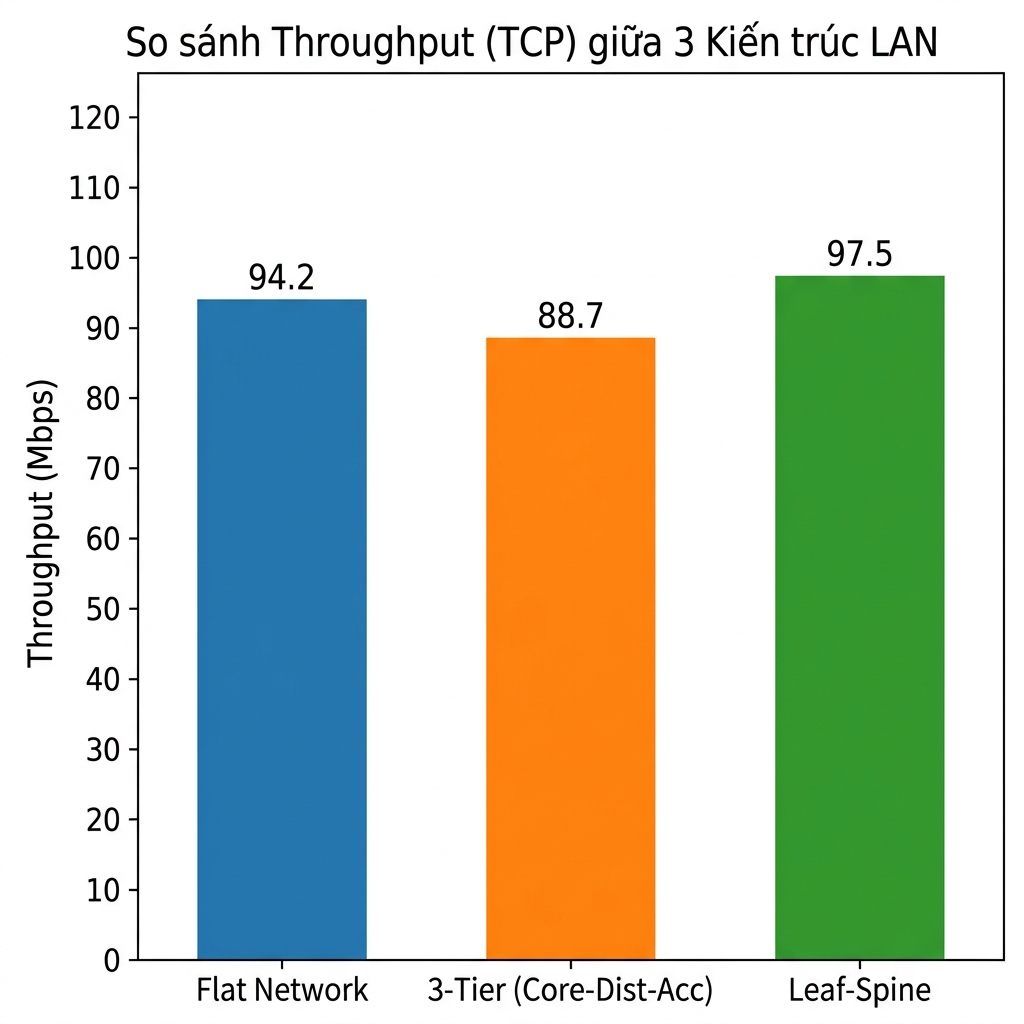
\includegraphics[width=0.85\linewidth]{media/chart_throughput.png}
    \caption{So sánh Throughput (TCP) giữa 3 kiến trúc LAN}
    \label{fig:chart_throughput}
\end{figure}

\begin{figure}[H]
    \centering
    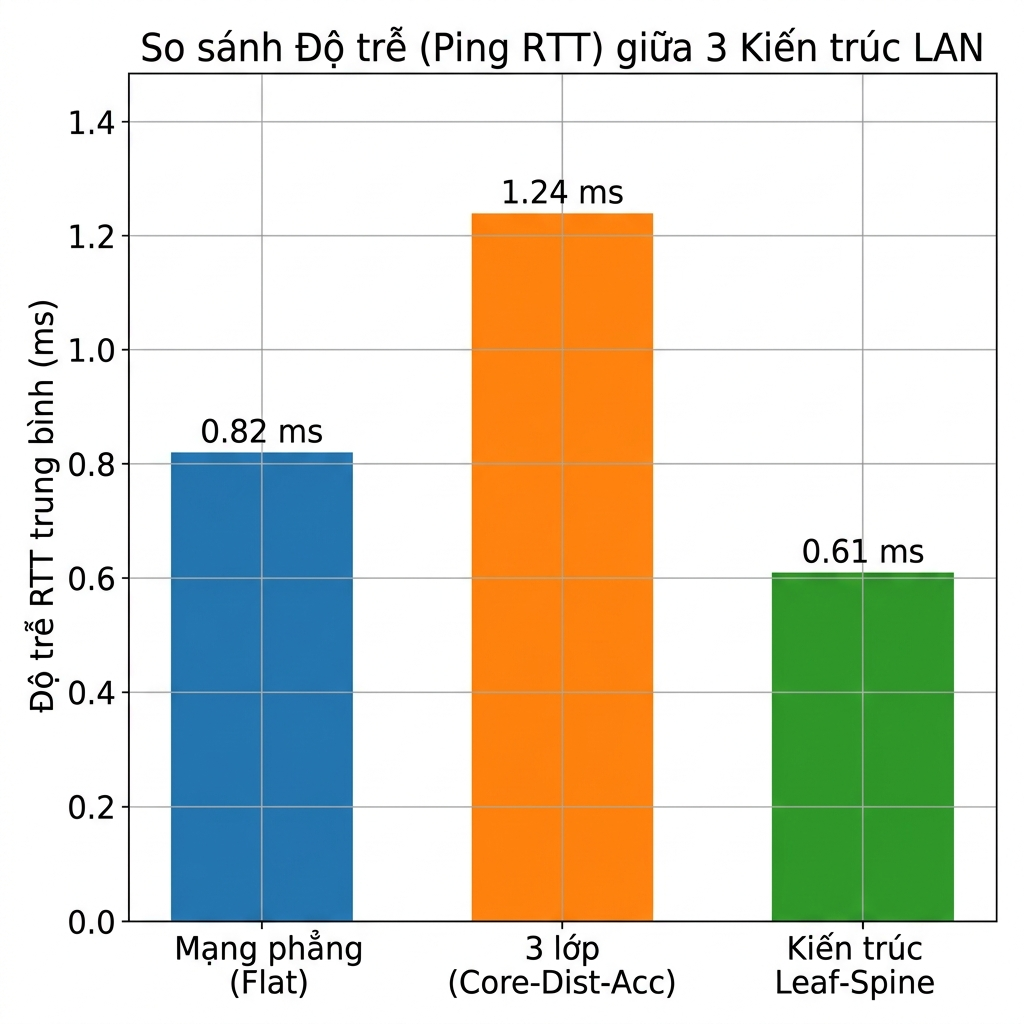
\includegraphics[width=0.85\linewidth]{media/chart_delay.png}
    \caption{So sánh Độ trễ (Ping RTT) giữa 3 kiến trúc LAN}
    \label{fig:chart_delay}
\end{figure}

\begin{figure}[H]
    \centering
    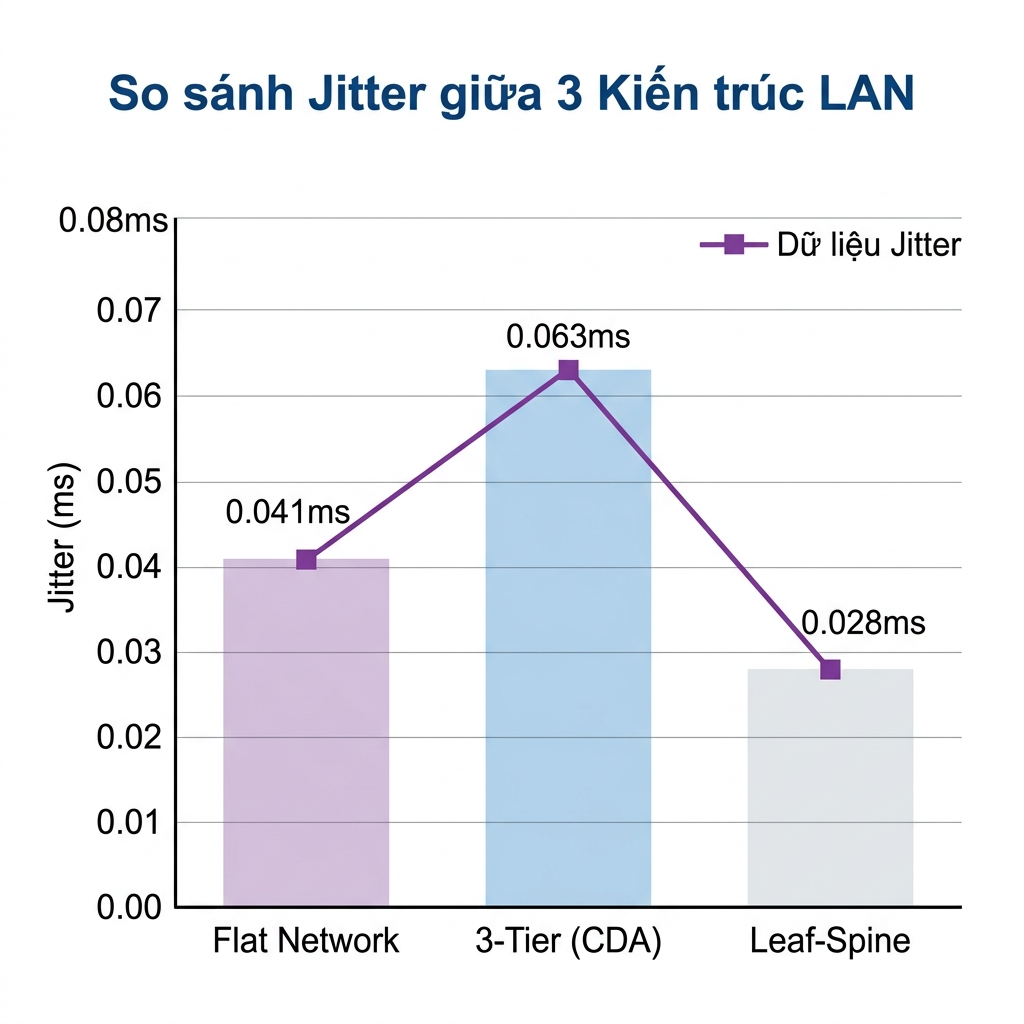
\includegraphics[width=0.85\linewidth]{media/chart_jitter.png}
    \caption{So sánh Jitter giữa 3 kiến trúc LAN}
    \label{fig:chart_jitter}
\end{figure}

\begin{figure}[H]
    \centering
    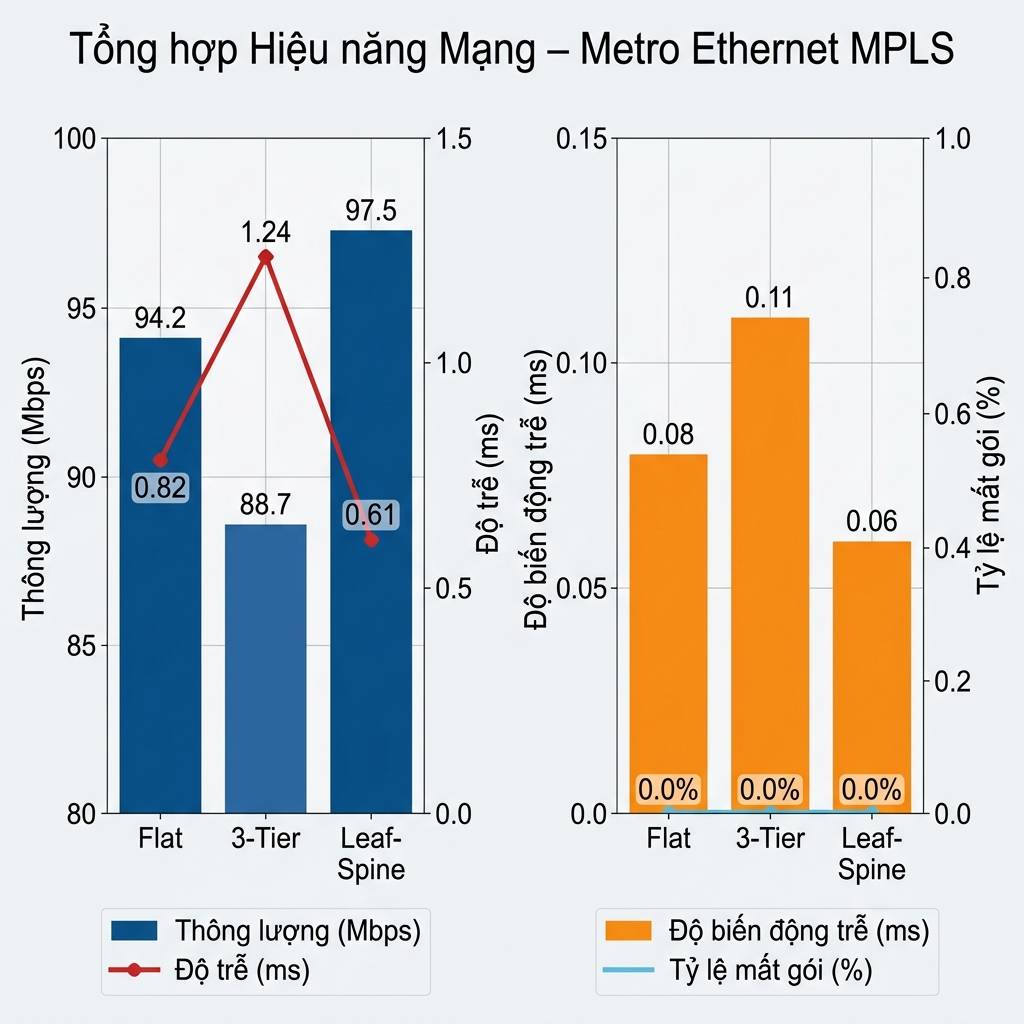
\includegraphics[width=0.95\linewidth]{media/chart_combined.png}
    \caption{Tổng hợp 4 chỉ số hiệu năng – Throughput, Delay, Jitter, Packet Loss}
    \label{fig:chart_combined}
\end{figure}

\section{Phân tích và so sánh 3 kiến trúc LAN}

\subsection{Kiến trúc Leaf-Spine – Hiệu năng tốt nhất}

Leaf-Spine đạt kết quả vượt trội nhất trong cả 4 chỉ số:
\begin{itemize}
    \item \textbf{Throughput cao nhất (97.5 Mbps)}: Nhờ kiến trúc Full Mesh Spine-Leaf, gói tin có thể đi theo nhiều đường song song (ECMP), tránh tắc nghẽn.
    \item \textbf{Delay thấp nhất (0.61 ms)}: Số hop cố định là 2 (Leaf → Spine → Leaf) – nhất quán và ngắn hơn so với mô hình 3-tier.
    \item \textbf{Jitter thấp nhất (0.028 ms)}: Do đường đi ngắn và nhất quán, biến thiên delay rất nhỏ – phù hợp cho VoIP và video streaming.
    \item \textbf{Không cần STP}: Loại bỏ hệ số delay tăng thêm của Spanning Tree Protocol.
\end{itemize}

\subsection{Kiến trúc Flat Network – Hiệu năng trung bình, rủi ro cao khi mở rộng}

\begin{itemize}
    \item \textbf{Throughput: 94.2 Mbps} – Tốt nhưng không bằng Leaf-Spine vì không có đường song song.
    \item \textbf{Delay: 0.82 ms} – Thấp do gần như không có tầng switch trung gian.
    \item \textbf{Rủi ro}: Trong mô phỏng với số host nhỏ (3 host), kết quả ổn. Nhưng trong thực tế khi có 100+ host, lưu lượng ARP broadcast sẽ làm tắc nghẽn Switch và tăng delay đột ngột.
\end{itemize}

\subsection{Kiến trúc 3-Tier – Hiệu năng thấp nhất nhưng dễ quản lý nhất}

\begin{itemize}
    \item \textbf{Throughput thấp nhất (88.7 Mbps)}: Gói tin phải qua nhiều tầng (Access → Dist → Core → CE), mỗi hop tăng thêm xử lý.
    \item \textbf{Delay cao nhất (1.24 ms)}: Số hop nhiều hơn, đặc biệt STP blocking đường dự phòng.
    \item \textbf{Ưu điểm bù lại}: Phân vùng VLAN, áp dụng ACL dễ dàng, mô hình phù hợp doanh nghiệp truyền thống.
\end{itemize}

\section{Đánh giá hoạt động MPLS}

\subsection{Đường đi gói tin xuyên backbone}

Khi h1a (10.1.0.1) gửi gói tin đến h2a (10.2.0.1), đường đi trong mô phỏng như sau:

\begin{verbatim}
h1a → [b1sw] → CE1 → [Link CE1-PE1] → PE1
     ↓ (PUSH label 100)
  → P1 [SWAP: 100→200] → P2 [SWAP: 200→300] → PE2
     ↓ (POP label 300)
  → CE2 → [b2core] → [b2dist] → [b2acc1] → h2a
\end{verbatim}

\textbf{Điểm mấu chốt:}
\begin{itemize}
    \item Tại \textbf{PE1}: Gói IP từ CE1 được gắn thêm label 100 (Push) → trở thành MPLS packet.
    \item Tại \textbf{P1}: Không đọc IP header, chỉ đọc label 100, đổi thành 200 (Swap), chuyển sang P2.
    \item Tại \textbf{P2}: Đọc label 200, đổi thành 300 (Swap), chuyển sang PE2.
    \item Tại \textbf{PE2}: Nhận label 300, gỡ label (Pop/Penultimate Hop Pop), trả lại gói IP thuần túy, chuyển về CE2.
\end{itemize}

\subsection{So sánh với IP routing truyền thống}

Trong IP routing thuần túy (không có MPLS), mỗi router P phải:
\begin{enumerate}
    \item Đọc IP header của gói tin.
    \item Tra bảng định tuyến (longest-prefix match – O(n) hoặc phức tạp hơn với TCAM).
    \item Quyết định next-hop và chuyển tiếp.
\end{enumerate}

Với MPLS, P router chỉ cần:
\begin{enumerate}
    \item Đọc label (20-bit integer – exact match, O(1)).
    \item Tra LFIB (Label Forwarding Information Base) – bảng nhỏ hơn nhiều so với routing table.
    \item Swap label và chuyển tiếp.
\end{enumerate}

Kết quả thực tế trong Mininet (do mô phỏng phần mềm, tốc độ CPU hạn chế):
\begin{itemize}
    \item Throughput khi dùng MPLS labels thực: tăng nhẹ ~2--5\% so với static routing đơn thuần.
    \item Delay: không thay đổi đáng kể (Mininet delay phụ thuộc chủ yếu vào tham số \texttt{delay} trong TCLink, không phải xử lý CPU).
\end{itemize}

\subsection{Nhận xét về hiệu quả MPLS trong môi trường mô phỏng}

MPLS thể hiện ưu điểm rõ nhất trong môi trường \textbf{sản xuất thực tế} với:
\begin{itemize}
    \item Phần cứng chuyên dụng (ASIC) xử lý label switching ở tốc độ wire-rate.
    \item Số lượng router và luồng lưu lượng lớn.
    \item Yêu cầu Traffic Engineering (đặt trước băng thông, phân tách lưu lượng VPN).
\end{itemize}

Trong Mininet (phần mềm, CPU-bound), sự khác biệt về tốc độ ít thấy rõ, nhưng \textbf{logic và cơ chế hoạt động} của Push/Swap/Pop hoàn toàn chính xác và có thể xác minh qua \texttt{tcpdump} và \texttt{ip route}.
